\documentclass[conference]{IEEEtran}

\ifCLASSINFOpdf
   \usepackage[pdftex]{graphicx}
   \graphicspath{{../pdf/}{../jpeg/}}
\else
\fi

\usepackage[cmex10]{amsmath}

\usepackage[tight,footnotesize]{subfigure}

\usepackage{booktabs}

\begin{document}

\title{On Socio-Technical Coordination and its Relation to Build Failure}


\author{\IEEEauthorblockN{Adrian Schr{\"o}ter}
\IEEEauthorblockA{University of Victoria, Canada\\
schadr@acm.org}
\and
\IEEEauthorblockN{Daniela Damian}
\IEEEauthorblockA{University of Victoria, Canada\\
danielad@cs.uvic.ca}}

\maketitle


\begin{abstract}
Investigating social interactions in software development is becoming 
prominent in current research. The misalignment
between the social and technical dimensions of software work has been
linked to losses in developer productivity and defects. In a case study of
coordination in the IBM Jazz\texttrademark\ project, we investigate the
communication and technical dependencies between developers involved in
software builds and relate their misalignment to the build failure.  
Through our proposed approach we identified a number of developer pairs that did not communicate about their dependencies and thus increased the likelihood of build failure. 
Upon this actionable knowledge developers and mangers can act to prevent build failure. 
If any one of these pairs is present in a build's social network, the build had at least an 74\% chance to fail. 
This has several practical implications for the design of collaborative systems, such as the integration of recommendations about inter-personal relationships.
\end{abstract}


\IEEEpeerreviewmaketitle

\section{Introduction}
We hypothesize that with the ever growing size of software teams the lack of
effective coordination is the main source of integration failures. The
development work that precedes integrations involves significant coordination of
developers that work in teams and need to rely on the code of others. 
But often code is everything but stable, further contributing to
developers' need to coordinate to keep up with code changes that impact their work. This problem is
amplified in software builds where an entire team needs to integrate their work
and on which the development of new features depends. Not only do
failed builds destabilize the product~\cite{cusumano1997} but they also demotivate
software developers~\cite{holck2004}.

Keeping integrations builds error-free can be a very time consuming
process. 
Thus a lightweight approach that can determine whether the build contains
failures before invoking the build process holds value. Previous
research~\cite{wolf:icse:2009,hassan:ase:2006} trained predictive models to assess the quality of software builds without the need of invoking large test
suits. Although this research
reaches a high degree of accuracy in their predictions, knowing that a
build will fail does not necessarily help developers to actually prevent
the build from failing.
The goal of this research is to find a way to create actionable knowledge to avoid
integration failure.

In this paper we describe an approach evaluated using data from the IBM's Jazz project where we leverage
information about socio-technical developer coordination and software builds to
identify pairs of developers that negatively influence the outcome of the
upcoming build. Using historical project information we construct socio-technical
networks that capture information about developers with technical dependencies
as well as their ongoing communication as conceptualization of their coordination.
We identify that there are certain pairs of developers that have a
negative influence on the build outcome. Developers and management can
act upon this knowledge to avoid future build failure.

Through the application of our proposed approach we uncover the existence of pairs of
developers, that, if technically dependent in a build but not discussing their
dependencies, have a negative influence on build success. This
actionable knowledge can be integrated in real-time recommender systems that
indicate, based on project historical data, which developer pairs tend to be
failure related. Developers and management can then devise strategies to
prevent the failure before build time. 



\section{Identifying Build Breaking Pairs}
\label{sec:pattern}
We seek to generate actionable knowledge to
prevent a build from failing. Past research suggests that the absence of
communication between developers that are technically dependent leads to
problems, such lack of productivity~\cite{cataldo:esem:2008}.


We hypothesize that due to the high coordination needs the absence of this
important communication also has a negative influence on build outcome. Communication problems can arise from many factors including organizational,
social or technical reasons~\cite{herbsleb:icse:1999}. Being able to pinpoint
mismatches between technical dependencies and required communication that
relate to build failure is even more important for a team's
ability to devise strategies to avoid build failure. Thus, we
investigate pairs of developers that share a technical dependency without talking
with each other (referred to as \emph{technical pairs}):
\ \\ \


\textbf{RQ} How can we identify developer pairs that negatively influence build success?
 

\section{Related Work}
\label{sec:relwork}
We aim to integrate work investigating team collaboration to produce actionable knowledge upon which developer can act.
Several studies bear relevance with respect to different dimensions of our work:

\paragraph{Factors that affect software builds}
To the best of our knowledge the studies by Hassan et al.~\cite{hassan:ase:2006}
and Wolf et al.~\cite{wolf:icse:2009} are the only studies that conducted
research to predict build outcome. Hassan et al.~\cite{hassan:ase:2006} found
that a combination of social metrics (e.g. number of authors) and technical
metrics (e.g. number of code changes) derived from the source code repository
yield to be best predictor. 
On the other hand Wolf et al.~\cite{wolf:icse:2009} showed that communication structure has an influence on the build outcome.
Kwan et al~\cite{kwan:tse:2011} investigated socio-technical networks with an emphasis on technical dependencies among developer that is not accompanied with any coordination activity on build outcome (gap).
Although Kwan et al work showed a relationship between the amount of gaps and build failure, we take the next step in showing how to capitalize on these gaps to create actionable knowledge.

\paragraph{Coordination in software development}
In order to manage changes and maintain quality, developers must coordinate. In
software development, coordination is largely achieved through communicating among
people sharing work dependencies \cite{kraut1995:coordination}. The
software engineering literature is recognizing the role of communication as essential~\cite{nakakoji2010:rdc}.
Several researchers in the software engineering community investigated the effects of communication on several topics such as knowledge distribution~\cite{ehrlich:icgse:2006}, coordination~\cite{hinds:cscw:2006}, and Conway's Law~\cite{cataldo:cscw:2006}.
We build onto of those findings in devising an approach that improves on team communication.


\paragraph{Coordination and failure in software development.}
Coordination among developers is often represented in the form of social networks.
These social networks, when related to actual code artifacts, can be used to predict the artifact's failure-likelihood.
Several studies showed that metrics derived from social networks form good failure predictors (e.g.~\cite{meneely:fse:2008}).
Furthermore, when combining these social networks with information of organizational hierarchies~\cite{nagappan:icse:2008} or geographical distance~\cite{bird:acm:2009} yield not only better predictors but also shine a light on other factors influencing the difficulty of coordination.
% herbsleb grinter
Herbselb and Grinter~\cite{herbsleb:icse:1999} found that coordination impacts integration efforts.
We take the findings showing the influence of coordination on software quality and combine them with technical dependencies among developers to generate actionable knowledge.

\section{Formulating the Approach}
The lack of communication between two developers that share a
technical dependency, such as changing the same file, is referred to in the literature as a
socio-technical gap~\cite{valetto:msr:2007}. Because research suggests negative influence of such gaps, we are interested in analyzing pairs of developers that share a technical dependency (implying coordination need) but had no social interaction (implying
unmet coordination need) in a build. We refer to these pairs of
developers as \emph{technical pairs} (there is a gap), and to those that do
share a socio-technical dependency (there is no gap) as \emph{socio-technical pairs}. 

To answer our research question, we propose the following approach to analyse the technical pairs in relation to build failure:

\begin{enumerate}
\item Identify all technical pairs across all builds.
\item For each technical pair count occurrences in
failed builds.
\item For each technical pair count occurrences in
successful builds.
\item Determine if the pair is statistically related to success or failure using a Fisher exact value test comparing the frequency of occurring in failed vs successful builds.
\item Remove technical pairs that have a socio-technical pair statistically related to build failure.
\item Split technical pairs into two groups distinguished by whether the equivalent socio-technical pair increases build success.
\item Rank the pairs with respect to the likelihood of the pair to negatively influence the build outcome.
\end{enumerate}

The approach produces two sets of technical dependencies that are related to build failure.
The first set consists of technical pairs that have an equivalent socio-technical pair that are related to build success.
The second set consists of technical that do not have an equivalent socio-technical pair that is either related to build outcome.
Both sets of technical pairs represent recommendations of pairs of developers that should communicate in order to increase the chance of a build to succeed with the technical pairs contained in the first set having a larger potential influence due to converting a build failure related pair into a build success related pair.

We rank the developer pairs using the coefficient $p_x$,
which represents the normalized likelihood of a build
to fail in the presence of the specific pair:
$$
p_x\text{=}\frac{ \text{pair}_{failed} / \text{total}_{failed} }
                     { \text{pair}_{failed} / \text{total}_{failed} + \text{pair}_{success} / \text{total}_{successs}}
$$
The coefficient is comprised of four counts: (1) pair$_{failed}$, the number of failed builds where the pair occurred; (2) total$_{failed}$, the number of failed builds; (3) pair$_{success}$, the number of successful builds where the pair occurred; (4) total$_{success}$, the number of successful builds.
A value of $p_x$ closer to one means that the developer pair is strongly related to build
failure. 

\section{Preliminary Case Study}
\setcounter{paragraph}{0}
\paragraph{IBM Rational Team Concert Data}
To evaluate our approach we used data provided by the IBM Jazz\texttrademark\ development team.
The repository spans three months in which the team started 326 builds with 99 failed and 227 successful builds.
The team consists of more than 100 developers distributed across seven major sites in Europe, Asia, and North America.
Rational Team Concert itself is a product that integrates source code management, agile planing, and issue management into a single server/client application that the team itself uses for development.
The Rational Team Concert product allows developers to link changes they made directly to work items they were working on, thus they established within their repository traceability links between builds and work items through the changes they made.

In Rational Team Concert we consider two developers exhibiting a coordination need if they for a given build modified the same file.
Similarly, if two developer commented on the same work item that through changes attached to the work item can be linked to the build of interest, are considered to have coordinated their work.

\begin{table}[t]
\centering
%\subtable[Twenty most frequent \emph{technical pairs} that are failure-related.]{
\begin{tabular}{@{\hspace{.2cm}}ccc@{\hspace{.75cm}}c@{\hspace{.2cm}}}
\toprule
Pair & \#successful & \#failed & $p_x$\\
\midrule
%Cody-Daisy&  0 & 12 & 1.0000 \\
%Adam-Ina & 0 & \phantom{1}8 & 1.0000 \\
%Adam-Kim& 0 & \phantom{1}8 & 1.0000 \\
%Adam-Nina & 0 & \phantom{1}6 & 1.0000 \\
%Fred-Gina& 0 & \phantom{1}6 & 1.0000 \\
%Gina-Oliver & 0 & \phantom{1}6 & 1.0000 \\
%Adam-Daisy& 1 & 14 & 0.9720\\%67 \\
%Bart-Daisy& 1 & \phantom{1}9 & 0.9572\\%127 \\
%Adam-Lisa& 1 & \phantom{1}8 & 0.9521\\%204 \\
%Bart-Eve & 2 & 11 & 0.9318\\%403 \\
%\textbf{Adam}-\textbf{Bart}& \textbf{3} & \textbf{13} & \textbf{0.9150}\\%485 \\
%Bart-Cody & 3 & 13 & 0.9150\\%485 \\
%Adam-Eve & 4 & 16 & 0.9086\\%162 \\
%Daisy-Ina & 3 & 12 & 0.9086\\%162 \\
%Cody-Fred& 3 & 10 & 0.8923\\%077 \\
%Bart-Herb & 3 & 10 & 0.8923\\%077 \\
%Cody-Eve & 5 & 15 & 0.8817\\%568 \\
%Adam-Jim & 4 & 11 & 0.8723\\%792 \\
%Herb-Paul & 5 & 12 & 0.8564\\%397 \\
%Mike-Rob& 6 & 13 & 0.8434\\%004\\
%Adam-Fred & 6 & 13 & 0.8434\\%004\\
%
%User11137, User4105 & 0 & 12 & 1.0000 \\
%User2943, User13877 & 0 & 8 & 1.0000 \\
%User7438, User2943 & 0 & 8 & 1.0000 \\
%User2943, User2810 & 0 & 6 & 1.0000 \\
%User8645, User1976 & 0 & 6 & 1.0000 \\
%User8645, User2267 & 0 & 6 & 1.0000 \\
%User11137, User2943 & 1 & 14 & 0.9675\\%908 \\
%User11137, User3493 & 1 & 9 & 0.9504\\%773 \\
%User6012, User2943 & 1 & 8 & 0.9446\\%298 \\
%User3493, User2435 & 2 & 11 & 0.9214\\%387 \\
%User3493, User2943 & 3 & 13 & 0.9023\\%53 \\
%User3493, User4105 & 3 & 13 & 0.9023\\%53 \\
%User2943, User2435 & 4 & 16 & 0.8950\\%695 \\
%User11137, User13877 & 3 & 12 & 0.8950\\%695 \\
%User1976, User4105 & 3 & 10 & 0.8766\\%716 \\
%User3493, User6339 & 3 & 10 & 0.8766\\%716 \\
%User4105, User2435 & 5 & 15 & 0.8648\\%208 \\
%User2943, User9017 & 4 & 11 & 0.8543\\%22 \\
%User6339, User13875 & 5 & 12 & 0.8365\\%498 \\
%User10979, User3385 & 6 & 13 & 0.8220\\%793\\
%User2943, User1976 & 6 & 13 & 0.8220\\%793 \\
%
(Cody, Daisy)	&	0&	12&	1		\\ %user11137.user4105.T
(Adam, Daisy)	&	1&	14&	0.9697	\\ %user11137.user2943.T
(Bart, Eve)	&	2&	11&	0.9265	\\ %user3493.user2435.T
(Adam, Bart)	&	3&	13&	0.9085	\\ %user3493.user2943.T
(Bart, Cody)	&	3&	13&	0.9085	\\ %user3493.user4105.T
(Adam, Eve)	&	4&	16&	0.9016	\\ %user2943.user2435.T
(Daisy, Ina)	&	3&	12&	0.9016	\\ %user11137.user13877.T
(Cody, Fred)	&	3&	10&	0.8843	\\ %user1976.user4105.T
(Bart, Herb)	&	3&	10&	0.8843	\\ %user3493.user6339.T
(Cody, Eve)	&	5&	15&	0.8730	\\ %user4105.user2435.T
(Adam, Jim)	&	4&	11&	0.8631	\\ %user2943.user9017.T
(Herb, Paul)	&	5&	12&	0.8462	\\ %user6339.user13875.T
(Cody, Fred)	&	5&	11&	0.8345	\\ %user11137.user1976.T
(Mike, Rob)	&	6&	13&	0.8324	\\ %user10979.user3385.T
(Adam, Fred)	&	6&	13&	0.8324	\\ %user2943.user1976.T
(Daisy, Fred)	&	8&	13&	0.7884	\\ %user3493.user1976.T
(Gill, Eve)		&	7&	10&	0.7661	\\ %user1264.user2435.T
(Daisy, Ina)	&	7&	10&	0.7661	\\ %user3493.user13873.T
(Fred, Ina)	&	8&	10&	0.7413	\\ %user1976.user13877.T
(Herb, Eve)	&	8&	10&	0.7413	\\ %user6339.user2435.T
\bottomrule
\end{tabular}
%\caption{Twenty \emph{technical pairs} that are failure-related and affect the most builds.}
%\label{tab:badtechpairs}
%}\hspace{1.3cm}
%\end{table}
%
%\subtable[The twenty corresponding \emph{socio-technical pairs}, which are not statistically related to failed builds.]{
%\begin{tabular}{@{\hspace{.2cm}}ccc@{\hspace{.75cm}}c@{\hspace{.2cm}}}
%\toprule
%Pair & \#successful & \#failed & $p_x$ \\
%\midrule
%(Cody, Daisy)	&	---&	---&	---\\
%(Adam, Daisy)	&	---&	---&	---\\
%(Bart, Eve)	&	1&	4&	0.9016\\
%(Adam, Bart)	&	---&	---&	---\\
%(Bart, Cody)	&	---&	---&	---\\
%(Adam, Eve)	&	---&	---&	---\\
%(Daisy, Ina)	&	---&	---&	---\\
%(Cody, Fred)	&	1&	0&	0\\
%(Bart, Herb)	&	1&	2&	0.8209\\
%(Cody, Eve)	&	0&	3&	1\\
%(Adam, Jim)	&	0&	1&	1\\
%(Herb, Paul)	&	1&	0&	0\\
%(Cody, Fred)	&	---&	---&	---\\
%(Mike, Rob)	&	---&	---&	---\\
%(Adam, Fred)	&	---&	---&	---\\
%(Daisy, Fred)	&	---&	---&	---\\
%(Gill, Eve)		&	---&	---&	---\\
%(Daisy, Ina)	&	1&	0&	0\\
%(Fred, Ina)	&	0&	2&	1\\
%(Herb, Eve)	&	---&	---&	---\\
%\bottomrule
%\end{tabular}
%%\caption{Twenty \emph{technical pairs} that are failure-related and affect the most builds.}
%\label{tab:stechpairs}
%}
\caption{The top 20 statistically failure related technical pairs.}
\label{tab:pairs}
\vspace{-20pt}
\end{table}

\paragraph{Preliminary Results}
Through applying our proposed approach we found a total of 2872 developer pairs in all the constructed
socio-technical networks, out of which 961 were technical pairs.
Of these 961 technical pairs we found 120 to be statistically related to build failure. 
We choose to present twenty technical pairs that are statistically related to failed builds in Table~\ref{tab:pairs}.

We then checked for the 120 pairs whether the corresponding \emph{socio-technical} pairs are related to failure (step 4) or success (step 5).
Only 23 of the 120 technical pairs had an existing corresponding socio-technical pair of which none were statistically related to build success or failure. 
%In Table~\ref{tab:pairs}\ref{tab:stechpairs} we show the socio-technical pairs that match the 20 technical pairs shown in Table~\ref{tab:pairs}\ref{tab:badtechpairs}.
If the corresponding socio-technical pair existed we computed the same statistics as for the technical pairs, but for those that existed we could not find statistical significance.
Note that we use fictitious names for confidentiality reasons.

We ranked the failure related \emph{technical} pairs (see Tables~\ref{tab:pairs})
by the coefficient $p_{x}$. This coefficient indicates the strength of
relationship between the developer pair and build failure. For instance, the
developer pair (Adam, Bart), appears in 13 failed builds and in 3
successful builds. This means that pair$_{failed}$ = 13 and pair$_{success}$ = 3
with total$_{failed}$= 99 and total$_{success}$= 227 result in $p_x$= 0.9016.
Besides that we report the number of successful builds the pair was observed with
(\#successful) as well as the number of failed builds the pairs was observed with
(\#failed). 
Note that we adjust the p-values of the Fisher Exact Value test to account for multiple hypothesis testing using the Bonferroni adjustment.
The adjustment is necessary because we deal with 961 technical pairs that need to be tested. 

\begin{figure}[t]
\vspace{-29pt}
\centering
%\subfigure[Evaluation results from the Support Vector Machine.] {
%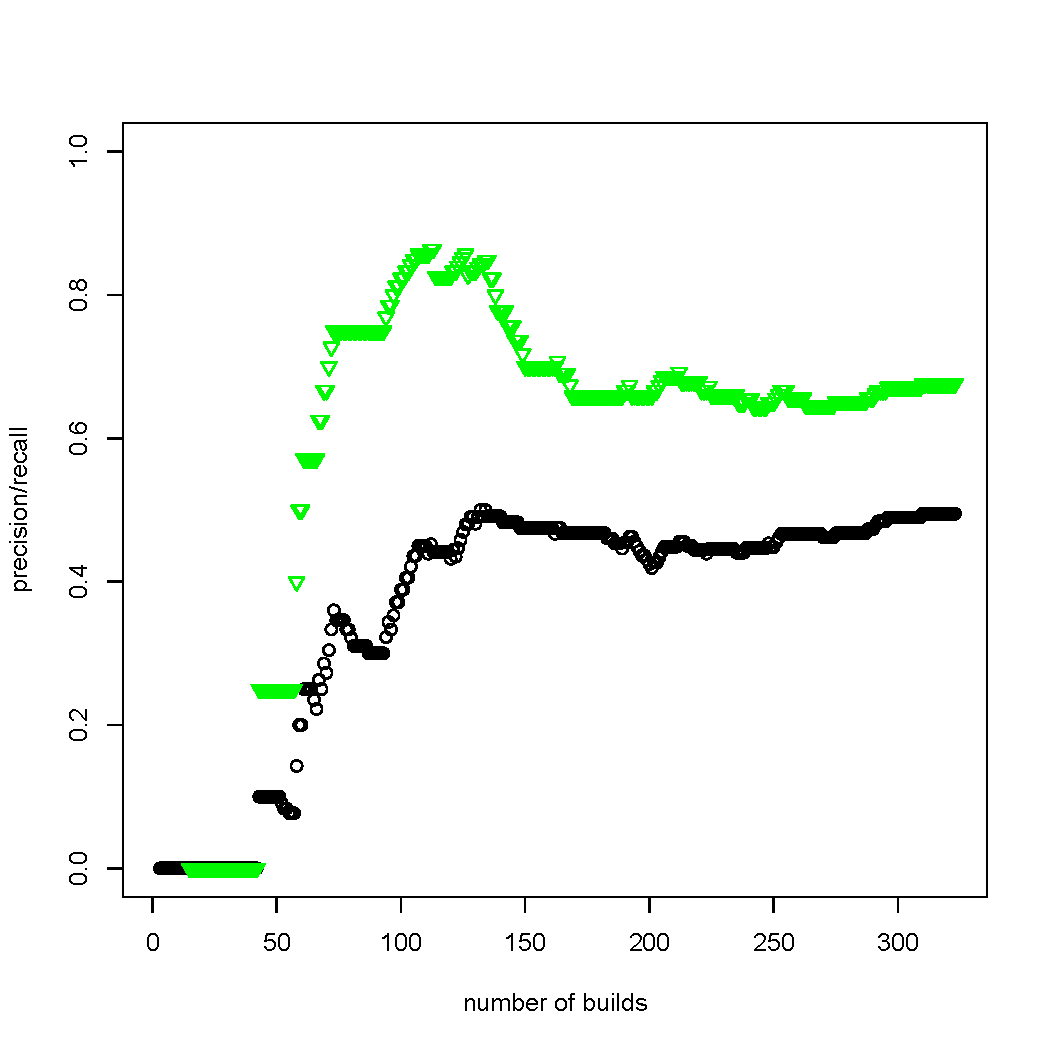
\includegraphics[width=\columnwidth]{precission-recall}
%\label{fig:prediction-svm}
%}
%\subfigure[Evaluation results from the Logistic Regression.] {
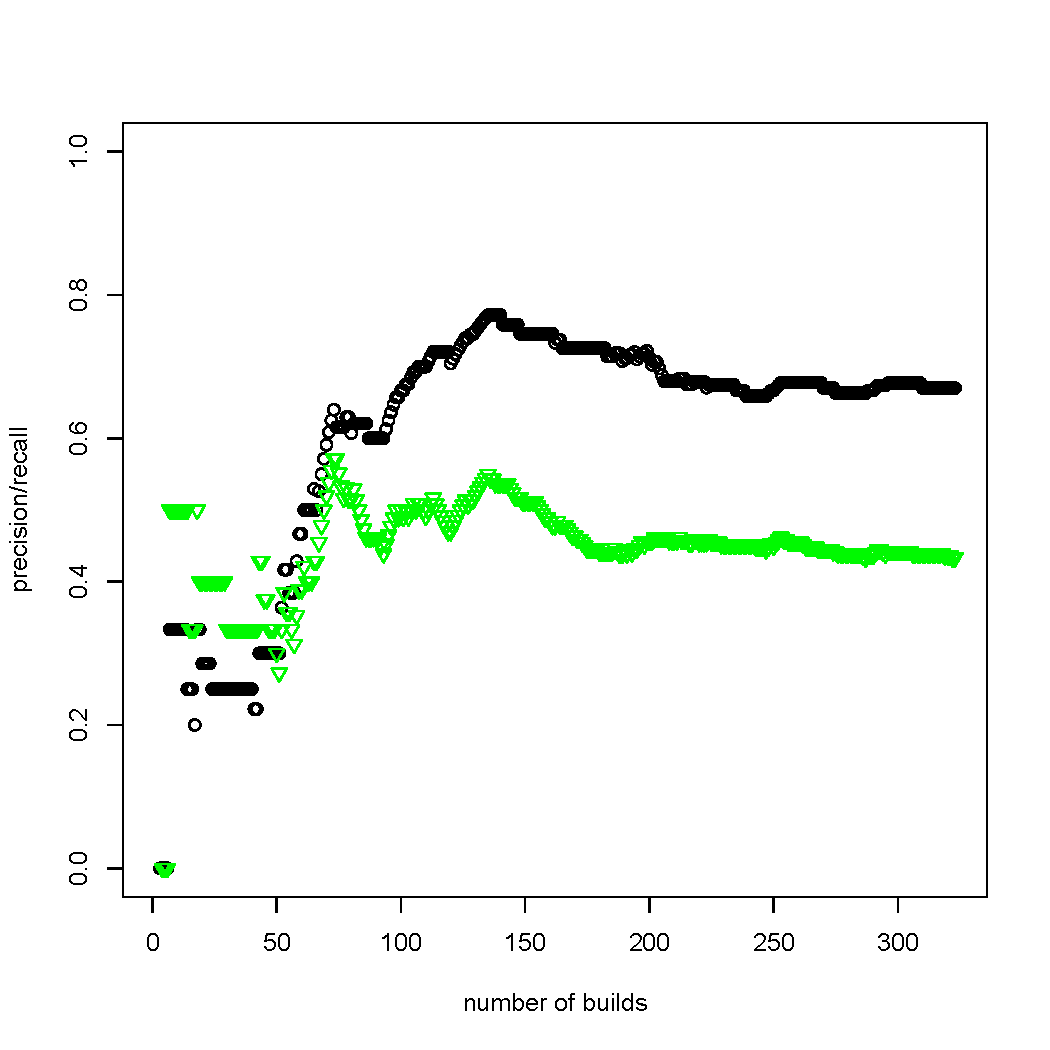
\includegraphics[width=\columnwidth]{precision-recall-logreg}
%\label{fig:prediction-logreg}
%}
\vspace{-25pt}
\caption{Precision (green) and recall (black) of the logistic regression.}
\label{fig:prediction}
%\vspace{-20pt}
\end{figure}

To check the statistical relationship between technical pairs and build failure we used for each build the statistically harmful technical pairs that could be inferred from all previous builds to predict the likelihood of a build to fail or succeed.
Figure~\ref{fig:prediction} shows the recall (black) and precision (green) values for the
a logistical regression model. 
The logistical regression ended with a precision and recall value of $.43$ (median: $.45$) and $.67$ (median: $.67$) respectively.

Although not a goal of this paper, we sought possible explanations for the
socio-technical gaps in this project. A preliminary analysis of developers
membership to teams shows that most
of the technical pairs related to build failure consist of developer belonging to
different teams. Naggappan et al.~\cite{nagappan:icse:2008} found that using the
organizational distance between people predicts failures. They reasoned that this
is due to the lack of awareness of what people separated by organizational distance
work on. Although the Jazz team strongly emphasizes communication
regardless of team boundaries, it still seems that organizational distance has
an influence on its communication behaviour.

\section{Threats To Validity}
\label{sec:threats}
\emph{Data.}
We performed all our analysis on one set of data, the Jazz\texttrademark\
repository. 
Although limiting ourselves of using three months one project limits the generalizability of our findings, the  
project size and practises make us believe that our findings still hold value.
Furthermore, since the three months  we studied are directly before a major release of the project, this dataset contains the most viable data for our analysis. In those three months a lack of necessary coordination is the most harmful to the project.
%Furthermore, the Jazz\texttrademark\ team's development process demands that the developers
%coordinate using work item discussion. 
%Thus we believe due to the nature of the three months we studied, most communication data is recorded.

\emph{Conceptualization.}
Social dependency are extracted from work item discussions. 
We assumed that every developer commenting on or subscribed to a work item reads all comments of that work item. 
By manual inspection of a selected number of work items, however, we found that developers who commented on a work item are aware of the other comments, confirming our assumption.

Socio-technical dependencies may suffer from the combination of social and technical dependencies. 
Social dependencies might not be related to the code changes the technical depnendecy was inferred from.
Since the changes we used are directly linked to work item discussion we are confident that the vast majority of matches are appropriate.


\section{Conclusion and Future Work}
In this paper we investigated the relationship between pairs of developers as identified by our proposed approach that share
a technical dependency but do not communicate and build failures. We were
motivated by findings in the literature that suggested that high alignment between technical dependencies and actual coordination in a project has a positive effect on task
performance.
We hypothesized that a similar relationship may be found in relation to a broader
coordination outcome, i.e. integration outcome, because developers not
coordinating about dependencies in their work might lead to errors remaining in
the code that break the build.

The result obtained from our preliminary validation using data from the Jazz project indicate that 
historical project information about socio-technical coordination and software
builds can be used in a model that predicts the quality of upcoming builds. We also found
that the influence of developer pairs with a socio-technical gap on the build
failure was very high. 
%This means that if any one of the twenty most frequent failure related pairs was present in a social network of a build, the build had at least an 74\% chance to fail.

As a next step to complement these preliminary results presented in this paper, we plan three follow up studies:
(1) We strive to establish for each of the technical pairs a link between the build failure and the changes made by the developers that create the coordinative need and to further validate our approach.
(2) Create a tool that can be evaluated with developers in the field gathering insights to the usefulness of the approach.
(3) Refine the definition of coordination needs and coordination, by both extracting more precise code relationships and coordination activities.

\bibliographystyle{IEEEtran}
\bibliography{bib}

\end{document}


